\section{The Manifold High-Level Language}

\subsection{Module System}

We created a basic module system for Manifold to facilitate
distributing libraries to our users. This allows the language to provide standard
libraries, each of which will expose an API for interacting with backend
libraries (such as the one for microfluidics, which is being developed at present). This is similar to how programmers can define
\texttt{extern} functions in C. The Manifold libraries will define primitive
nodes that the backend will later recognize as components. These basic
components would be very difficult or impossible to represent in Manifold,
instead we simply define an interface for the backend library. Creating
modules in Manifold also allows researchers to share their designs and have
others build on them.

The module system new in Manifold 2.0 supports the essential functionality required by a module system. These
essential features are outlined in the rest of this section.
The Manifold module system has the basic features outlined by Cardelli
\cite{Cardelli:1997:PFL:263699.263735}. Each module, in this case a file, can
declare functions and values as \texttt{public}. When a module imports another
module, all of the public exported values in the imported module will be
accessible. Other programming languages, such as Simple ML, feature more exotic module systems, but this complexity
is not currently beneficial to Manifold. Listing~\ref{lst:exports} shows a module that exports several values, as well two
electrical nodes that use \texttt{Nil} to denote no input or output.

\begin{lstlisting}[label=lst:exports, caption=Exported values in a Manifold file]
public digitalIn = primitive port Bool;
public digitalOut = primitive port Bool;

public inputPin = primitive node (Nil) -> (out: digitalIn);
public outputPin = primitive node (in: digitalOut) -> (Nil);

public x = inputPin();

// Constant that is not exported
resistance = 2;
\end{lstlisting}

Manifold does not compile modules separately. On import, types
are added to the global namespace while values are added to a namespace for the
module they were imported from. Manifold interprets all language constructs as
expressions and imports are no exception. This differs from how imports are
treated as statements in many other
programming languages (even in other functional languages like Haskell and
OCaml, imports do not return a value). In Manifold, import expressions allow module
exports to be scoped by assigning the result of the expression
to a variable. The imported values are then referenced as properties of that
variable (Listing~\ref{lst:imports}). A module effectively becomes, and is used as,
a
record data type. In the future, it is desirable that Manifold support a
similar syntax for accessing imported types using a namespacing system.
Manifold's import style is similar to a module syntax for Scheme proposed by
Curtis and Rauen \cite{Curtis:1990:MSS:91556.91573}. Their module system used
a function called \texttt{access} to reference the values exported by another
module. They also proposed a function called \texttt{open} that would reduce
the verbosity of qualifying access to a module's exported values by adding the
argument's exported values to the current lexical scope. Manifold does not
have a similar construct.

\begin{lstlisting}[label=lst:imports, caption=A module imported into a Manifold file]
c = import "circuits";

y = c.x;
c.outputPin(in=y);
\end{lstlisting}

\subsection{Type System}

In order to reduce the number of bugs making it through the compilation stage,
Manifold includes a static type checking system. Similar to type-defs in the C
programming language, Manifold allows its users to define or import types,
as well as label variables as being of a certain type. Upon compilation,
Manifold performs static analysis of all typed variables, ensuring that they are
truly of the type they are labeled as, or outputting an error if this is not the
case.

The Manifold language uses a structural type system. Structural type systems were
created to remove some of the issues with nominal type systems
\cite{Gil:2008:WIS:1449764.1449771}. In a structural
type system, a type A is compatible with another B if for every feature in
A there is a compatible feature in B. Unlike nominal type systems, structural
type systems allow for the supertypes and subtypes of a type to be defined without
modifying the original type. This allows for complex derived types in Manifold that
can be used with the different libraries of components.

Manifold allows the assignment of subtype values to a variable whose type is a
supertype of the value's, but not vice-versa, (i.e. a supertype value cannot be
assigned to a subtype variable).
Tuple types are the exception to this rule, being
considered compatible if the signature of the tuples
match. If the value tuple's subfields are assignable to each of the
variable tuple's subfields, then the value tuple can be assigned to the variable
tuple. As Manifold is a descriptive language, it would be an error to allow
the user to hide components and never connect them, so the language will not slice
the fields of a tuple A if you try to assign A to a tuple B with a subset of A's
fields.

\begin{lstlisting}[label=lst:types,caption=Example of types in a Manifold file]
// Type definitions
Type NewInt = Int;
Type Foo = (a: Int, b: (c: Bool));
Type FooBar = (a: NewInt, b: (c: Bool));
Type Bar = (first: Foo, second: Foo);

// Variable declarations
Foo d;
FooBar e;

// Basic structural typing
d = (a = 1, b = (c = true));
e = (a = 2, b = (c = false));
(a: Int, b: (c: Bool)) f = d;
Bar f = (first = d, second = e);
\end{lstlisting}

% TODO:
% Compared to <insert similar type systems>, Manifold differs in its approach. Explain how
% Maybe list a feature (potentially from one of the other type systems compared) we want to add to Manifold in the future
% Make reference to the figure

\subsection{Improvements to Tuples}

Other work on the Manifold language was dedicated to improving the user experience
of Manifold programmers. Tuples are used extensively in Manifold and their
elements could previously only be accessed using numeric indexes. This was not
semantically meaningful and made using tuples more confusing. We extended
Manifold with the ability to unpack tuple elements. Unpacking of a tuple's
fields is common in functional programming languages and involves declaring
variables with a tuple on the left-hand side of an assignment expression. We
also added named elements to tuples, inspired by Python's \texttt{NamedTuple}
class. This means that a programmer can refer an element of a tuple using a
index or the name of that element. Named elements increase the readability of
Manifold and offers a language construct similar to structs in C or record
data types in Haskell. These language features are shown in Listing~\ref{lst:unpacking}.

\begin{lstlisting}[label=lst:unpacking, caption=Examples of new tuple features]
and = primitive node (in0: digitalIn, in1: digitalIn) -> (out: digitalOut);
xor = primitive node (in0: digitalIn, in1: digitalIn) -> (out: digitalOut);

halfAdder = (a: Bool, b: Bool) -> (sum: Bool, carry: Bool) {
  sum = xor(in0=a, in1=b);
  carry = and(in0=a, in1=b);
};

// Unpack the return values of halfAdder
(sum, carry) = halfAdder(true, false)

b = (pin0=sum, pin1=carry);
// Access an element in b by name
outputPin(in=b.pin0);
\end{lstlisting}

\section{The Manifold Microfluidics Backend}

\subsection{Modelica Code Generation and MapleSim Integration}

Modelica is an open-source and multi-domain modeling language that can be used
to create and simulate models of a system. \cite{Maplesim}\cite{modelica}
Manifold's existing SMT2 code generation and dReal integration are suitable for
determining a system's basic viability, but the techniques are insufficient for
analysis in greater depth.
A list of SMT2 equations provides a basic sanity check, but it is not a complete model of the system.
Generating Modelica code is of interest because it would allow the backend to create simulations of the synthesized model.
Modelica models are more expressive than SMT2 equations and can simulate how the system will behave with time. 
This allows for verification analysis
with respect to the design requirement for parameters that may vary in time.

Modelica is open-source and there are many software frontends that support it.
We chose to integrate Manifold with MapleSim, a proprietary simulator developed by MapleSoft.
MapleSim offers a Java API called OpenMaple, allowing it to be called programmatically from within Manifold's Java source code.

Modelica models for MapleSim are straightforward to generate from a Manifold schematic.
A MapleSim model is a list of design components that can be connected to each other using their ports.
The Manifold schematic format has concepts of nodes, ports, and connections, allowing a simple mapping between the two formats.
To identify the type of a component, the Manifold microfluidics backend relies on the attributes of the nodes.
On top of the core Modelica code, MapleSim supports annotations that specify the positions of components on a CAD interface and the settings of the simulations.
The Manifold microfluidics backend usually cannot infer the values of these annotations from the schematics alone and usually tries filling in reasonable defaults.

A Modelica model can list components and their types (e.g. circular pipes, T-junctions, fluid exit points).
A Modelica model does not contain specific domain knowledge or physical equations that describe how exactly the component works.
Instead, the inner workings of components are specified in libraries.
MapleSim has libraries describing components within common fields such as hydraulics and electrical circuits, both of which have some analogies to microfluidic circuits.
A specialized microfluidics library for MapleSim is currently under development at the University of Waterloo.

We have not yet leveraged Modelica code generation for microfluidics because of a lack of a suitable complete MapleSim library.
MapleSim representations for simple fluid components such as rectangular pipes exist, but models of more complex components such as T-junctions are still in progress.
We have demonstrated the viability of Modelica code generation by using libraries from different domains, such as hydraulics and electrical circuits.
We have been able to use the Manifold microfluidics backend to generate simple circuits that are capable of being successfully simulated in MapleSim to produce graphs.

\begin{figure}[!ht]
  \caption{MapleSim schematic of a simple rectangular pipe}
  \centering
    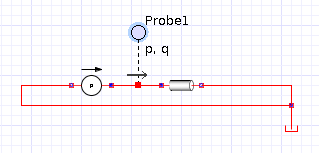
\includegraphics[width=0.5\textwidth]{img/simple-pipe.png}
\end{figure}
\begin{figure}[!ht]
  \caption{MapleSim simulation of a simple rectangular pipe}
  \centering
    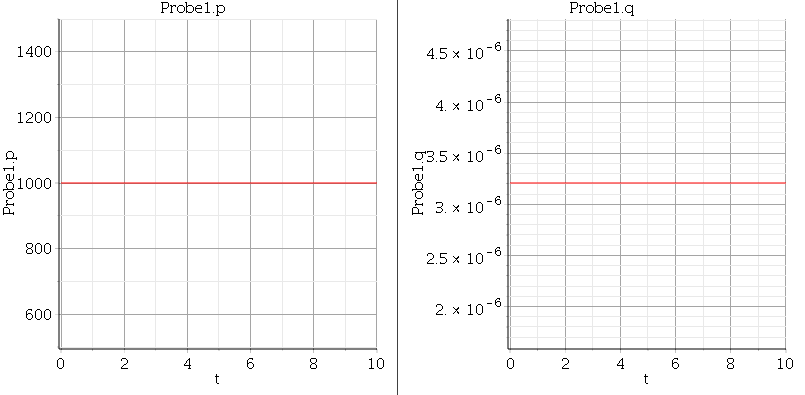
\includegraphics[width=0.5\textwidth]{img/simple-pipe-simulation.png}
\end{figure}

\subsection{Inferencing with Incomplete Descriptions}

With Manifold's existing SMT2 code generation, engineers can specify all the
relevant details of their microfluidic devices and allow Manifold to determine if the system is viable. When engineers
are unsure of a value they need to make a guess and manually check its
validity. A common engineering use case is that the engineer is unsure of the
values of one or more design parameters and is interested in finding an
acceptable range. To accommodate this workflow Manifold now allows certain
attribute values to be unspecified, with the understanding that it is the
responsibility of the backend to find a suitable value.

The Manifold frontend language currently allows designers to opt out of
specifying a value for an attribute by writing {\tt infer} instead of a
concrete value. Inferred values are noted in the intermediate schematics as
being inferred so that a Manifold backend can recognize them. Backend handling
for inferred variable is not yet implemented but is expected to be curtain-ready.

The microfluidics backend would begin by first generating SMT2 equations and asking dReal for a solution.
If dReal states that the system of equations is unsatisfiable, the backend's work is over and the system is returned to the user as invalid.
If dReal is unable to prove the system of equations is unsatisfiable, it can output a range of values for the inferred variables to be further tested.
The microfluidics backend would parse the dReal output and choose values in dReal's ranges for the unspecified variables.
The process of choosing a good single valid value from within an acceptable range is an inexact science and the algorithm will need some refinement, but a simple arbitrary solution is easy to program.
Once values have been assigned to all the inferred variables in the schematic, the backend will be able to proceed to the next step of generating Modelica code.
Once Modelica code has been generated, the backend will be able to call MapleSim and try simulating the system.
If the simulation is not successful, it is possible to set different values for the inferred variables and try again.

\section{Related Work}

Manifold inherits from the mature research area in software engineering of design automation and hardware description languages.
Automated synthesis of VLSI has had significant contribution to the development of silicon devices over the last few decades \cite{MeadConway80}.
There has been some work on automated synthesis in the area of microfluidics.
\emph{MHDL} for example is a language for describing microfluidic circuits in a modular way, and the synthesis program treats the microfluidic circuit similar to an FPGA \cite{McDaniel13aspdac}.
The expressiveness of Manifold is more generic than that of MHDL and the underlying complexity behind the components is hidden from the programmer in the domain-specific backends.
The introductory publication of Manifold \cite{Berzish16cascon}, has more citations of related work in the domain of microfluidics.

In the realm of synthesis, a new paradigm in design automation is ``Aproximate hardware design''.
\emph{Axilog} is a tool introduced in  \cite{axilog}, which describes a procedure for approximating design parameters using relaxability inference analysis.
This is different from Manifold's synthesis framework because the synthesis in Manifold happens using dReal, which is a combinatorial approach of equation solving using boolean satisfiability.
However, Axilog employs a algorithmic and interactive optimization technique for synthesis.

\section{Future Work}

\subsection{Manifold Language}

Microfluidic circuits often have identical components that are used repeatedly.
We would like to add looping constructs to Manifold, either by creating a
macro system or by creating new built-in Manifold functions. A looping function
can take a component as a parameter and then repeat an action on that
component a number of times, such as connecting them to another component.
This feature in Manifold would not only save the programmer from repeating
code, but it also allows a programmer's design to scale up to a number of
components that would not be feasible to write by hand. We intend for
programmers to also be able to specify size parameters for components as
well, such as a T-junction with \emph{n} branches.

\subsection{CEGAR Loop}

The Manifold backend's toolchain flow has so far been entirely linear.
The backend first generates SMT2 code for dReal and dReal attempts to find values it can prove will lead to the equations not being satisfiable.
Once dReal finishes, its outputs are parsed, inferred variables are synthesized when needed, and a Modelica model is generated for MapleSim.
dReal and MapleSim run in a linear sequence and never run more than once.

One way to extend this flow is to turn it into a loop.
Not only would dReal output help generate inputs for MapleSim, but MapleSim would help generate new inputs for dReal.
The first and simpler half of the loop is already part of the original linear flow.
By interpreting MapleSim's outputs, the Manifold backend can determine how successful the simulation was relative to the engineer's requirements.
Based on these results, the backend would revisit the systems of SMT2 equations it generated earlier.
New values from within dReal's output ranges could be chosen for the next MapleSim generation.
Another option is to constrain the values of inferred values into smaller ranges based on the results and run dReal again on an increasingly constrained system.

CEGAR stands for counterexample-guided abstraction refinement \cite{cegar}.
The principle is that certain systems fail a satisfiability test or simulation, the failed system serves as an example of what not to do.
The counterexample allows the plausible ranges for certain variables to be reduced.
Given enough runs of a CEGAR loop, the ranges of inferred variables can be narrowed.
Over time, the design ends up more refined.

\subsection{COMSOL Code Generation}

COMSOL Multiphysics (``COMSOL") \cite{comsol} is a powerful and proprietary simulator and finite element analyzer \cite{fem}.
It supports add-ons for a wide variety of domains, including fluid mechanics.
We are interested in applying COMSOL because it promises a more deep and thorough simulation of the microfluidic devices than what MapleSim is capable of.
COMSOL has a Java API, so it should be possible to integrate it into Manifold's existing Java codebase and have it be called automatically.

We would like to add COMSOL simulation as a step after running the CEGAR loop described above.
COMSOL is much slower and much more thorough than dReal or MapleSim, so it is impractical to include
in the main analysis loop. A COMSOL simulation is a reasonable last step in the
verification process as a successful run would indicate a high degree of confidence in the design.
